% Capítulo 5 - Resultados
% devem ser apresentados, de forma objetiva, precisa e clara, tanto os resultados positivos quanto os negativos que foram obtidos com o desenvolvimento do trabalho, sendo feita uma discussão que consiste na avaliação circunstanciada, na qual se estabelecem relações, deduções e generalizações.

\chapter{Resultados}
\begin{figure}
  \centering
    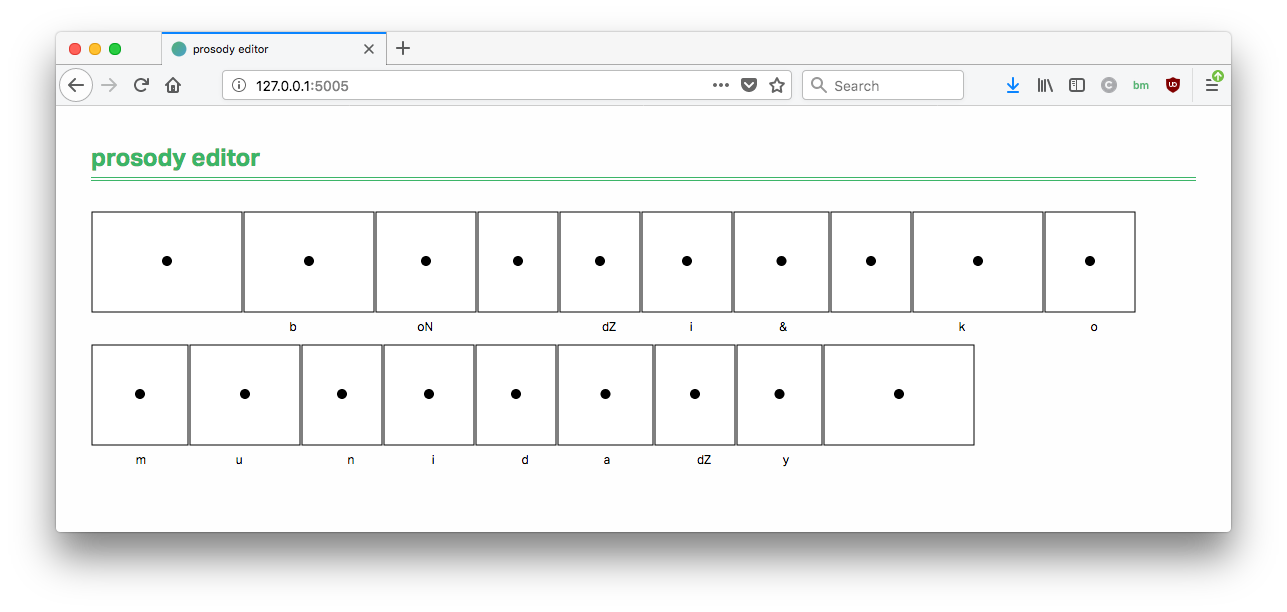
\includegraphics[width=1\textwidth]{Imagens/editor.png}
  \caption{Editor gráfico desenvolvido}
  \label{fig:ed}
\end{figure}

Com o levantamento dos sistemas TTS desenvolvidos para o português brasileiro, é
possível observar que há carência de suporte à síntese expressiva. Seguindo o
modelo de funções prosódicas de \citeonline{taylor2009}, os sistemas estudados
concentram-se na geração de prosódia suprassegmental, mas não há suporte algum à
geração de prosódia afetiva e aumentativa atualmente.

Linguagens de marcação como SSML e EmotionML já começaram a ser integradas a
\emph{frameworks open-source} e sistemas comerciais de TTS para múltiplas
línguas, mas não foram encontrados trabalhos para o português brasileiro.

Estudando os modelos de anotação entoacional, percebe-se que ainda não há uma
solução considerada mais apropriada para analisar o português brasileiro. Há,
por outro lado, uma grande quantidade de trabalhos de análise de contornos
melódicos que podem ser futuramente adaptados e convertidos em parâmetros para
sistemas TTS expressivos, servindo como base para a geração manual ou automática
de prosódia afetiva.

Identificamos lacunas que precisam ser preenchidas, como a criação de corpus
anotados prosodicamente e algoritmos de compreensão textual para geração de
marcação EmotionML.

Com o desenvolvimento dos programas para linha de comandos e para \emph{web}
neste trabalho, dá-se um passo inicial para a melhoria de prosódia afetiva e
aumentativa em sistemas TTS para o português brasileiro.
